\documentclass[german,12pt]{article}

\author{Michael Klopsch}
\newcommand{\spectitle}[1]{\title{Nutzterdokumentation -- Buchschloss -- #1}}

\usepackage{babel}
\usepackage{xcolor}
\usepackage[hidelinks]{hyperref}
\hypersetup{linktoc=all}
\usepackage{graphicx}
\usepackage{enumitem}
\usepackage[titles]{tocloft}

\addtolength{\cftsubsecnumwidth}{10pt}  % with tocloft, https://tex.stackexchange.com/questions/296545

\widowpenalties 1 10000  % https://tex.stackexchange.com/questions/21983

\makeatletter % https://tex.stackexchange.com/questions/8351/what-do-makeatletter-and-makeatother-do
\renewcommand*{\fps@figure}{hbtp} % https://tex.stackexchange.com/questions/364817/how-to-change-default-float-options-for-figures
\g@addto@macro\@floatboxreset\centering % https://tex.stackexchange.com/questions/2651/should-i-use-center-or-centering-for-figures-and-tables
\makeatother

\addtolength{\topmargin}{-0.8in}
\addtolength{\textheight}{1in}

\renewcommand{\thesection}{\Roman{section}}
\renewcommand{\thesubsubsection}{\thesubsection.\Alph{subsubsection}}

\newcommand{\linkandref}[2]{\hyperref[#1]{#2}\footnote{Siehe Abs. \ref{#1} auf S. \pageref{#1}, }}
\newcommand{\hinweis}[1]{\begin{quote}\textbf{Hinweis}: #1\end{quote}}
\newcommand{\figref}[1]{Abb. \ref{#1}}


\spectitle{Graphische Oberfläche (gui2)}

\begin{document}

\maketitle
\newpage

\tableofcontents
\newpage

\section{Schnellstart}
\label{sec:quickstart}
\subsection{Ein neues Buch erstellen}
\label{subsec:quickstart:new_book}
Ein Mitglied, welches mindestens Supermitarbeiter ist, kann neue Bücher erstellen. Dazu klicken wir zuerst auf ``neu'', dann auf ``Buch''. Es erscheint eine lange Liste mit Daten, die benötigt werden. 
Aber keine Angst: nach Eingabe der ISBN muss hoffentlich nicht mehr viel gemacht werden.

Sobald wir das Eingabefeld der ISBN mit der Tab-Taste oder durch Klicken auf ein anderes Feld verlassen, wird gefragt,
ob einige Daten automatisch von der Deutschen Nationalbibliothek abgefragt werden sollen (dazu ist eine Internetverbindung notwendig).
Nachdem wir ``Ja'' gewählt haben, werden nach max. einigen Sekunden im besten Fall viele Felder ausgefüllt.
Einige müssen wir jedoch noch selbst füllen (z.B. das Regal) oder ggf. anpassen (z.B. die Serie aus dem Titel entfernen).

Scheitert die Autofüllung, wird eine Fehlermeldung angezeigt. Handelt es sich um einen Verbindungsfehler, sollte die Internetverbindung überprüft werden. Wurde die ISBN nicht gefunden, sollte die ISBN auf Tippfehler untersucht werden.

Wenn alle (nötigen) Felder gefüllt sind, klicken wir auf ``Durchführen'', um das Buch anzulegen.
Falls es Fehler bei der Verarbeitung gab, wird eine Fehlermeldung gezeigt. Ansonsten erscheint eine Benachrichtigung, welche die Identifikationsnummer des Buches beinhaltet.
Diese sollte so früh wie möglich in oder auf das Buch gebracht (geschrieben, geklebt, ...) werden.

\subsection{Ein Buch als ausgeliehen vermerken}
\label{subsec:quickstart:borrow}
Um ein Buch als ausgeliehen zu vermerken, wählen wir ``ausleihen''. Wir geben dann die ID des Buches in das entsprechende Feld ein. Kommt der jetzt ausleihende Schüler unten vor, drücken wir auf den entsprechenden Knopf, um das Buch auszuleihen. Ansonsten müssen wir erst die Schülerausweisnummer des ausleihenden Schülers eintragen.

\hinweis{ Bei Bedarf kann auch die Ausleihdauer angepasst werden. Die Zahl ist die Ausleihdauer in Wochen.}

\subsection{Ein Buch als zurückgegeben vermerken}
\label{subsec:quickstart:restitute}
Wird ein Buch zurückgegeben, drücken wir auf ``zurückgeben''. Jetzt müssen wir die Felder für die Buch-ID und die Schülerausweis-Nr. ausfüllen.
Dann drücken wir auf ``Durchführen''. Bei Problemen wird eine Fehlermeldung angezeigt.

\hinweis{ Die Schülerausweisnummer wird abgefragt, um Probleme durch Vertippen bei Eingabe der Buch-ID zu verhindern. 
Sollte nicht bekannt sein, wer ein Buch ausgeliehen hat, kann dies durch die \linkandref{subsubsec:detail:view:book}{``betrachten'' $\rightarrow$ ``Buch''-Aktion} eingesehen werden.
Alternativ ist es in der Textoberfläche möglich, eine Rückgabe durchzuführen, ohne dass eine Schülerausweis-Nr. benötigt wird.}

\section{Die Oberfläche}
\label{sec:interface}
\subsection{Die Infoleiste}
\label{subsec:interface:header}
\begin{figure}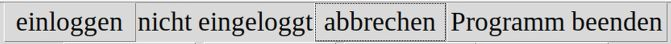
\includegraphics{images/gui2/head_not_logged_in.jpg}\caption{Die Infoleiste, wenn man nicht eingeloggt ist}\label{fig:head_not_logged_in}\end{figure}

Die Infoleiste (\figref{fig:head_not_logged_in}) befindet sich immer am oberen Bildschirmrand.
Sie enthält Login-Informationen sowie mit ``Abbrechen'' und ``Programm beenden'' beschriftete Knöpfe.

\begin{figure}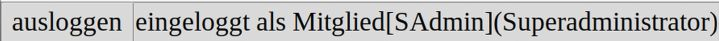
\includegraphics{images/gui2/logged_in_info.jpg}\caption{Information, wenn man eingeloggt ist}\label{fig:logged_in_info}\end{figure}
\begin{figure}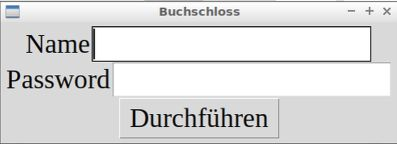
\includegraphics{images/gui2/login_form.jpg}\caption{Felder zum Einloggen}\label{fig:login_form}\end{figure}

Oben links befindet sich ein Knopf, der zu Ein- und Ausloggen dient.
Neben diesem befindet sich ein kurzer Text, der anzeigt, ob und wie man derzeit eingeloggt ist (s. \figref{fig:logged_in_info}). 
Zum Einloggen muss der Knopf gedrückt werden, dann müssen die entsprechenden Daten in die jeweiligen Felder (s. \figref{fig:login_form}) eingegeben werden.

Mit Klick auf den ``Abbrechen''-Knopf wird der mittlere Teil des Fensters in seine Ausgangsposition, d.h. das erste Menü (s. \figref{fig:initial_menu}), zurückgesetzt.

Wenn man auf den ``Programm beenden''-Knopf klickt, wird das Programm nach einer Bestätigungsabfrage beendet. Falls während des Betriebs ein unerwarteter Fehler aufgetreten ist, hat man die Möglichkeit, eine Fehlermeldung per E-Mail an Michael zu schicken.

\subsection{Der Aktionsbereich}
\label{subsec:interface:action_center}
In der Mitte des Bildschirms befindet sich der Aktionsbereich. Was hier gezeigt wird, ändert sich, je nach dem, was man macht.
Generell wird entweder ein Menü, also mehrere Knöpfe, die zur Aktionsauswahl führen, oder eine einzelne Aktion, in der meist Eingaben zu machen sind, gezeigt.

\begin{figure}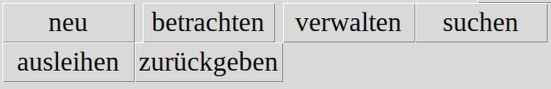
\includegraphics{images/gui2/initial_menu.jpg}\caption{Das erste Menü: hier kann man aus Unteraktionen wählen}\label{fig:initial_menu}\end{figure}
\begin{figure}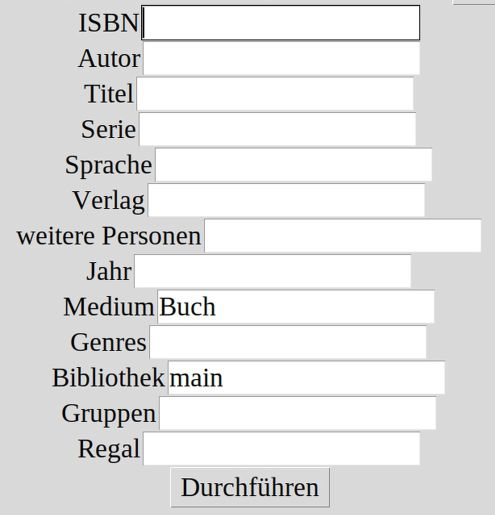
\includegraphics{images/gui2/new_book.jpg}\caption{Aktionsbeispiel Bucherstellung: hier werden Daten eingetragen}\label{fig:new_book_example}\end{figure}

Die meisten Aktionen bestehen daraus, Daten in Eingabefelder einzutragen bzw. bereits eingetragene Daten zu ändern. Danach wird mit Druck auf einen Knopf, meist mit ``Durchführen'' beschriftet, bestätigt. Siehe als Beispiel dazu \figref{fig:new_book_example}.

\section{Wie man was macht}
\label{sec:howto}
Da einige Aktionen nicht ganz intuitiv sind, werden hier Situationen zusammengefasst, wobei auf die jeweilige genaue Beschreibug verlinkt wird

\begin{minipage}{\textwidth} % needed for footnotes
\begin{tabular}{|p{0.5\textwidth}|p{0.4\textwidth}|}\hline
\begin{center}Situation\end{center} & \begin{center}Aktion\end{center}\\
\hline
ein Buch einer Bibliothek hinzufügen oder aus einer Bibliothek entfernen &\linkandref{subsubsec:detail:edit:book}{ ``verwalten'' $\rightarrow$ ``Buch''} oder \linkandref{subsubsec:detail:edit:library}{``verwalten'' $\rightarrow$ ``Bibliothek''} \\
\hline
mehrere Bücher einer Bibliothek hinzufügen oder aus einer Bibliothek entfernen & \linkandref{subsubsec:detail:edit:library}{``verwalten'' $\rightarrow$ ``Bibliothek"}\\
\hline
ein Buch einer Gruppe hinzufügen oder aus einer Gruppe entfernen & \linkandref{subsubsec:detail:edit:book}{``verwalten'' $\rightarrow$ ``Buch''} oder \linkandref{subsubsec:detail:edit:group}{``verwalten'' $\rightarrow$ ``Gruppe''} \\
\hline
mehrere Bücher einer Gruppe hinzufügen oder aus einer Gruppe entfernen & \linkandref{subsubsec:detail:edit:group}{``verwalten'' $\rightarrow$ ``Gruppe''}\\
\hline
alle Bücher einer Gruppe in eine Bibliothek bewegen & \linkandref{subsubsec:detail:edit:activate_group}{``verwalten'' $\rightarrow$ ``Gruppe aktivieren''}\\
\hline
Bestätigen, dass ein Schüler bezahlt hat & \linkandref{subsubsec:detail:edit:person}{``verwalten'' $\rightarrow$ ``Schüler''}\\
\hline
\end{tabular}
\end{minipage}

\section{Die einzelnen Aktionen im Detail}
\label{sec:detail}

Im Folgenden werden alle Aktionen genau beschrieben. Daher eignet sich dieser Bereich besonders zum Nachschlagen.

\subsection{``neu''}
\label{subsec:detail:new}
Diese Aktion wird verwendet, um neue Objekte zu erstellen.

\begin{figure}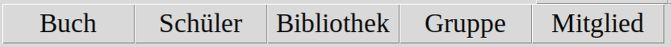
\includegraphics{images/gui2/new_menu.jpg}\caption{Unteraktionen für ``neu''}\label{fig:new_menu}\end{figure}

\subsubsection{``Buch''}
\label{subsubsec:detail:new:book}
\begin{figure}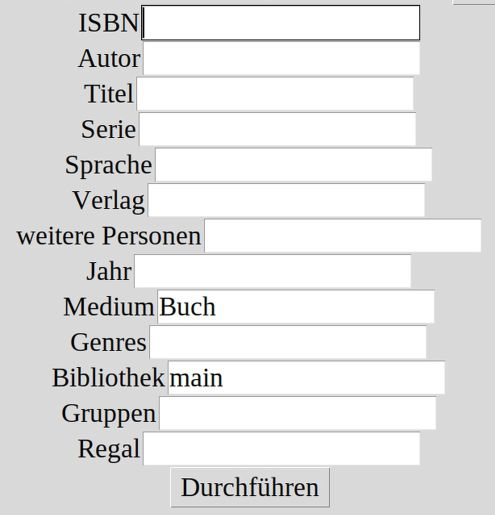
\includegraphics{images/gui2/new_book.jpg}\caption{Die Bucherstellung}\label{fig:new_book}\end{figure}

Mit dieser Aktion wird ein neues Buch erstellt. Die Aktionsoberfläche besteht aus den folgenden Eingabefeldern sowie dem ``Durchführen''-Knopf, mit dem die Aktion durchgeführt wird.
Um ein neues Buch zu erstellen, muss man mindestens Supermitarbeiter sein.

\begin{tabular}{|p{0.2\textwidth}|p{0.6\textwidth}|p{0.1\textwidth}|}\hline
\begin{center}Feld\end{center} & \begin{center}Bemerkung\end{center} & \begin{center}Muss angegeben werden\end{center}\\
\hline
ISBN & Die ISBN des Buches. Es werden SBN-, ISBN-10- und ISBN-13-Formate akzeptiert, jedoch intern in ISBN-13 umgewandelt. Die Prüfziffer wird geprüft. & Ja\\
\hline
Autor & Autor des Buches, bestenfalls im Format \verb=<Nachname>, <Vorname>= & Ja\\
\hline
Titel & Der Titel des Buches & Ja\\
\hline
Serie & Ggf. der Serienname. Bitte nicht zusätzlich im Titel angeben & Nein\\
\hline
Sprache & Die Sprache des Buches & Ja\\
\hline
Verlag & Der Verlag des Buches. & Ja\\
\hline
weitere Personen & Personen, die am Buch mitgewirkt haben, z.B. Illustratoren oder Übersetzer, bestenfalls im Format \verb=<Nachname-1>, <Vorname-1>: <Rolle-1>;= \ldots \verb=<Nachname-N>, <Vorname-N>: <Rolle-N>= & Nein\\
\hline
Jahr & Erscheinungsjahr als Zahl & Ja\\
\hline
Medium & Medium des Objekts, z.B. Buch, Heft, CD & Ja\\
\hline
Genres & Genres des Buches, bestenfalls aus einer Liste gewählt und mit Semikolon getrennt & Nein\\
\hline
Bibliothek & Gültige virtuelle Startbibliothek des Buchs, ohne besonderen Anlass ``main'' & Ja\\
\hline
Gruppen & Ggf. gültige Gruppen des Buches, mit Semikolon getrennt & Nein\\
\hline
Regal & Regal des Buches & Ja\\
\hline
\end{tabular}

\paragraph{Das Autofüllverhalten}
\begin{figure}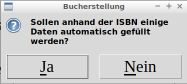
\includegraphics{images/gui2/ask_isbn_autofill.jpg}\caption{Es wird gefragt, ob Daten automatisch gefüllt werden sollen}\label{fig:ask_isbn_autofill}\end{figure}

Bewegt man sich aus dem ISBN-Feld heraus, wird, sofern die eingegebene ISBN eine gültige Länge hat und die Prüfziffer stimmt, gefragt, ob einige Daten automatisch gefüllt werden sollen.
Dies geschieht mittels einer Anfrage an die \href{https://portal.dnb.de}{Deutsche Nationalbibliothek}.
Wird das Buch gefunden, werden die erhaltenen Daten, meist Titel, Autor, Erscheinungsjahr, Sprache und Verlag, automatisch eingefüllt.

\hinweis{Es kann dazu kommen, dass die Oberfläche einige Sekunden lang nicht reagiert, während die Daten heruntergeladen werden. Dies wird erwartet und ist kein Problem.}

\hinweis{Bei einigen Datensätzen gibt es keine separaten Informationen zum Autor. Der Name ist meist im Titel vorhanden und kann durch Schneiden und Einfügen an die richtige Stelle gebracht werden. Ebenfalls kann die Serie im Titel auftauchen; auch sie sollte dann in das entsprechende Feld umgetragen werden.}

\subsubsection{``Schüler''}
\label{subsubsec:detail:new:person}
\begin{figure}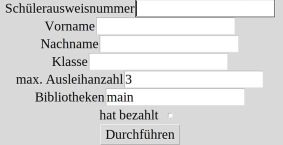
\includegraphics{images/gui2/new_person.jpg}\caption{Schülererstellung}\label{fig:new_person}\end{figure}

Mit dieser Aktion wird ein neuer Schüler erstellt. Die Aktionsoberfläche besteht aus den folgenden Eingabefeldern sowie dem ``Durchführen''-Knopf, mit dem die Aktion durchgeführt wird.
Um einen neuen Schüler zu erstellen, muss man mindestens Administrator sein; um eine maximale Ausleihanzahl über 3 zu erlauben Superadministrator.

\begin{tabular}{|p{0.2\textwidth}|p{0.6\textwidth}|p{0.1\textwidth}|}\hline
\begin{center}Feld\end{center} & \begin{center}Bemerkung\end{center} & \begin{center}Muss angegeben werden\end{center}\\
\hline
Schüler\-ausweis\-nummer & Die Schülerausweisnummer als Zahl & Ja\\
\hline
Vorname & Vorname des Schülers & Ja\\
\hline
Nachname & Nachname des Schülers & Ja\\
\hline
Klasse & Klasse des Schülers & Ja\\
\hline
max. \mbox{Ausleihanzahl} & Wie viele Bücher der Schüler gleichzeitig ausleihen darf & Ja\\
\hline
Bibliotheken & gültige Bibliotheken, zu denen der Schüler Zugang hat, mit Semikolon getrennt & Nein\\
\hline
hat bezahlt & Ob der Schüler bezahlt hat &   ---\\
\hline
\end{tabular}

\subsubsection{``Bibliothek''}
\label{subsubsec:detail:new:library}
\begin{figure}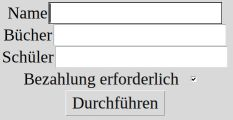
\includegraphics{images/gui2/new_library.jpg}\caption{Bibliothekserstellung}\label{fig:new_library}\end{figure}

Mit dieser Aktion wird eine neue Bibliothek erstellt. Die Aktionsoberfläche besteht aus den folgenden Eingabefeldern sowie dem ``Durchführen''-Knopf, mit dem die Aktion durchgeführt wird.
Um eine neue Bibliothek zu erstellen, muss man mindestens Administrator sein.

\begin{tabular}{|p{0.2\textwidth}|p{0.6\textwidth}|p{0.1\textwidth}|}\hline
\begin{center}Feld\end{center} & \begin{center}Bemerkung\end{center} & \begin{center}Muss angegeben werden\end{center}\\
\hline
Name & Der Name der Bibliothek; sollte kein Semikolon enthalten und eine vernünftige Länge haben & Ja\\
\hline
Bücher & Die IDs der Bücher, die sofort in die neue Bibliothek verlegt werden sollen, mit Semikolon getrennt & Ja\\
\hline
Schüler & Die Schülerausweisnummern der Schüler, die sofort Zugang zur neuen Bibliothek erhalten sollen, mit Semikolon getrennt & Ja\\
\hline
Bezahlung erforderlich & Ob Bezahlung erforderlich ist, um aus dieser Bibliothek auszuleihen &  ---\\
\hline
\end{tabular}

\hinweis{ Um alle Bücher einer Gruppe hinzuzufügen, muss man dies nach der Erstellung über \linkandref{subsubsec:detail:edit:activate_group}{``verwalten'' $\rightarrow$ ``Gruppe aktivieren''} machen.}

\subsubsection{``Gruppe''}
\label{subsubsec:detail:new:group}
\begin{figure}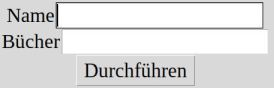
\includegraphics{images/gui2/new_group.jpg}\caption{Gruppenerstellung}\label{fig:new_group}\end{figure}

Mit dieser Aktion wird eine neue Gruppe erstellt. Die Aktionsoberfläche besteht aus den folgenden Eingabefeldern sowie dem ``Durchführen''-Knopf, mit dem die Aktion durchgeführt wird.
Um eine neue Gruppe zu erstellen, muss man mindestens Administrator sein.

\begin{tabular}{|p{0.2\textwidth}|p{0.6\textwidth}|p{0.1\textwidth}|}\hline
\begin{center}Feld\end{center} & \begin{center}Bemerkung\end{center} & \begin{center}Muss angegeben werden\end{center}\\
\hline
Name & Der Name der Gruppe; sollte kein Semikolon enthalten und eine vernünftige Länge haben & Ja\\
\hline
Bücher & Die IDs der Bücher, die sofort der neuen Gruppe hinzugefügt werden sollen, mit Semikolon getrennt & Nein\\
\hline
\end{tabular}

\subsubsection{``Mitglied''}
\label{subsubsec:detail:new:member}
\begin{figure}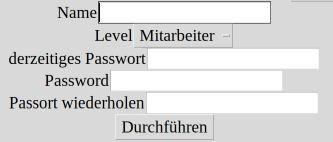
\includegraphics{images/gui2/new_member.jpg}\caption{Mitgliedserstellung}\label{fig:new_member}\end{figure}

Mit dieser Aktion wird ein neues Mitglied erstellt. Die Aktionsoberfläche besteht aus den folgenden Eingabefeldern sowie dem ``Durchführen''-Knopf, mit dem die Aktion durchgeführt wird.
Um ein neues Mitglied zu erstellen, muss man Superadministrator sein.

	\begin{tabular}{|p{0.2\textwidth}|p{0.6\textwidth}|p{0.1\textwidth}|}\hline
\begin{center}Feld\end{center} & \begin{center}Bemerkung\end{center} & \begin{center}Muss angegeben werden\end{center}\\
\hline
Name & Der Name des neuen Mitglieds & Ja\\
\hline
Level & Welche Berechtigungsstufe das Mitglied haben soll &  ---\\
\hline
derzeitiges Passwort & Das Passwort des z.Z. eingeloggten Mitglieds & Ja\\
\hline
Passwort & Das Passwort des neuen Mitglieds & Ja\\
\hline
Passwort wdh. & Eine Wiederholung des Passworts des neuen Mitglieds, um Tippfehler im Passwort zu vermeiden & Ja\\
\hline
\end{tabular}

\hinweis{Es wird empfohlen, dass das neue Mitglied möglichst bald alleine sein Passwort ändert oder es bei der Erstellung selbst eingibt.}

\subsection{``betrachten''}
\label{subsec:detail:view}
\begin{figure}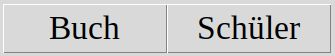
\includegraphics{images/gui2/view_menu.jpg}\caption{Unteraktionen für ``betrachten''}\label{fig:view_menu}\end{figure}

Mit dieser Aktion kann man sich Daten zu Schülern oder Büchern anzeigen lassen.

\subsubsection{``Buch''}
\label{subsubsec:detail:view:book}
\begin{figure}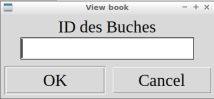
\includegraphics{images/gui2/view_book_ask.jpg}\caption{Die ID des Buches wird abgefragt}\label{fig:view_book_ask}\end{figure}

Nach Klick auf den Knopf wird man dazu aufgefordert, die ID des Buches anzugeben.

Danach wird eine Übersicht mit folgenden Informationen gezeigt:

\begin{tabular}{|p{0.3\textwidth}|p{0.6\textwidth}|}\hline
\begin{center}Feld\end{center} & \begin{center}Bemerkung\end{center}\\
\hline
Informationen zu & Die verkürzte Darstellung des Buches\\
\hline
ISBN & Die ISBN des Buches, im ISBN-13-Format\\
\hline
Autor, Titel, Serie, Verlag, Jahr, Medium, Sprache, weitere Personen, Genres, Bibliothek, Regal & Bei Erstellung des Buches bzw. bei der letzten Änderung angegebene Daten ohne Formatsänderung\\
\hline
ID & ID des Buches\\
\hline
Gruppen & Gruppen, in denen das Buch ist; mit Semikolon getrennt\\
\hline
Status & 
\begin{itemize}[leftmargin=*]
\item ``verfügbar'', wenn das Buch vorhanden ist
\item ``entliehen'', wenn das Buch derzeit entliehen ist
\item ``gelöscht'', wenn das Buch als gelöscht markiert wurde und nicht mehr entliehen werden kann
\end{itemize}
\\
\hline
Rückgabedatum & ggf. das Datum, bis zu dem das Buch spätestens zurückgegeben werden muss\\
\hline
entliehen von & ggf. eine Kurzdarstellung des Schülers, der das Buch entliehen hat; zeigt bei Klick mehr Informationen zum Schüler\\
\hline
\end{tabular}

\subsubsection{``Schüler''}
\label{subsubsec:detail:view:person}
\begin{figure}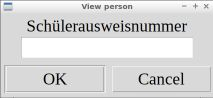
\includegraphics{images/gui2/view_person_ask.jpg}\caption{Die Schülerausweisnummer wird abgefragt}\label{fig:view_person_ask}\end{figure}

Nach Klick auf den Knopf wird man dazu aufgefordert, die Schüler\-ausweis\-nummer des Schülers anzugeben.

Danach wird eine Übersicht mit folgenden Informationen gezeigt:

\begin{tabular}{|p{0.4\textwidth}|p{0.5\textwidth}|}\hline
\begin{center}Feld\end{center} & \begin{center}Bemerkung\end{center}\\
\hline
Informationen zu & Die verkürzte Darstellung des Schülers\\
\hline
Schülerausweisnummer, Vorname, Nachname, Klasse, max.~Ausleihanzahl & Die bei Erstellung bzw. der letzten Änderung eingegebenen Daten\\
\hline
Bibliotheken & Bibliotheken, zu denen der Schüler Zugang hat, mit Semikolon getrennt\\
\hline
ausgeliehene Bücher & Bücher, die der Schüler derzeit ausgeliehen hat; mit Klick werden weitere Informationen zum Buch angezeigt\\
\hline
Bezahldatum & letztes Datum, an dem der Schüler bezahlt hat\\
\hline
\end{tabular}

\subsection{``verwalten''}
\label{subsec:detail:edit}
\begin{figure}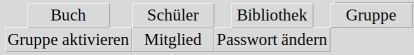
\includegraphics{images/gui2/edit_menu.jpg}\caption{Unteraktionen für ``verwalten''}\label{fig:edit_menu}\end{figure}

Mit dieser Aktion können Daten geändert werden

\subsubsection{``Buch''}
\label{subsubsec:detail:edit:book}
\begin{figure}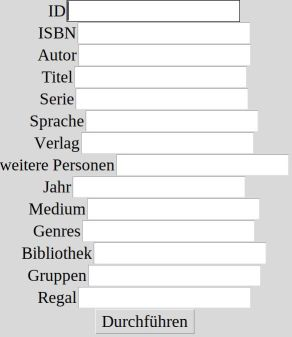
\includegraphics{images/gui2/edit_book.jpg}\caption{Die Buchverwatung}\label{fig:edit_book}\end{figure}

In der Buchverwaltung ist die Oberfläche der der Bucherstellung sehr ähnlich. Lediglich das Feld ``ID'' existiert zusätzlich.

Nach Eingabe der ID des zu verwaltenden Buches und Verlassen des Eingabefelds, etwa mit Klick auf ein anderes, werden die übrigen Felder automatisch mit den bereits vorhandenen Daten gefüllt.
Danach können Änderungen vorgenommen werden. Diese werden anschließend mit Klick auf ``Durchführen'' bestätigt.

\hinweis{In der Textoberfläche ist es möglich, Bücher als gelöscht zu markieren. Diese Möglichkeit gibt es in der graphischen Oberfläche nicht.}

\subsubsection{``Schüler''}
\label{subsubsec:detail:edit:person}
\begin{figure}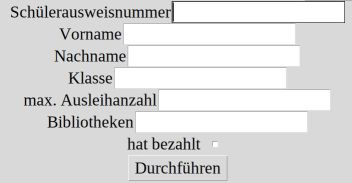
\includegraphics{images/gui2/edit_person.jpg}\caption{Die Schülerverwatung}\label{fig:edit_person}\end{figure}

Die Eingabefelder sind denen der Erstellung gleich. Nach Eingabe der Schülerausweisnummer und Verlassen des Eingabefelds werden die übrigen Felder automatisch mit den bereits vorhandenen Daten gefüllt.
Zusätzlich zu den Eingabefelder gibt es auch das ``hat bezahlt'' Häckchenfeld. Es soll gewählt werden, falls der Nutzer am Tag der Änderung bezahlt hat.

\hinweis{ In der Textoberfläche ist es möglich, ein beliebiges Bezahldatum festzulegen.}

\subsubsection{``Bibliothek''}
\label{subsubsec:detail:edit:library}
\begin{figure}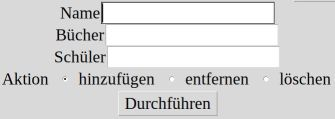
\includegraphics{images/gui2/edit_library.jpg}\caption{Die Bibliotheksverwatung}\label{fig:edit_library}\end{figure}

Im Bibliotheksverwaltungsbereich befinden sich folgende Eingabefelder:

\begin{tabular}{|p{0.2\textwidth}|p{0.6\textwidth}|p{0.1\textwidth}|}\hline
\begin{center}Feld\end{center} & \begin{center}Bemerkung\end{center} & \begin{center}Muss angegeben werden\end{center}\\
\hline
Name & Der Name der Bibliothek & Ja\\
\hline
Bücher & Die IDs der Bücher, mit denen Änderungen vorgenommen werden sollen, mit Semikolon getrennt & Nein\\
\hline
Schüler & Die Schülerausweisnummern der Schüler, mit denen Änderungen vorgenommen werden sollen, mit Semikolon getrennt & Nein\\
\hline
\end{tabular}

Zusätzlich befindet sich darunter ein Auswahlbereich, in dem die Art der Aktion (``hinzufügen", ``entfernen", ``löschen"), gewählt werden kann. Welche was bewirkt wird im Folgenden näher erläutert.

\paragraph{``hinzufügen''}
Mit dieser Aktion werden alle angegebenen Bücher in die angegebene Bibliothek gebracht, d.h. sie sind ab sofort in der angebenen Bibliothek, egal, in welcher Bibliothek sie vorher waren. Außerdem erhalten alle angegebenen Schüler Zugang zur angegebenen Bibliothek.

\hinweis{Wenn gleiche Bücher öfters die Bibliothek wechseln müssen, kann es sinnvoll sein, diese in eine Gruppe zusammenzufassen. Siehe dazu auch \linkandref{subsubsec:detail:edit:activate_group}{``Gruppe aktivieren''}}

\paragraph{``entfernen''}
Mit dieser Aktion werden alle angegebenen Bücher aus der angegebenen Bibliothek entfernt und in die Bibliothek ``main'' gebracht. Alle angegebenen Schüler verlieren Zugang zur angegebenen Bibliothek.

\hinweis{ Wenn die Bücher in eine andere Bibliothek verschoben werden sollen, kann dies direkt passieren, indem die Zielbibliothek angegeben und als Aktion ``hinzufügen'' gewählt wird.

}
\paragraph{``löschen''}
Mit dieser Aktion werden alle sich in der Bibliothek befindlichen Bücher zurück in die Bibliothek ``main'' gebracht und alle Schüler, die Zugang zur Bibliothek hatten, verlieren diesen. Die Eingabefelder ``Bücher'' und ``Schüler'' werden in diesem Fall ignoriert.

\hinweis{Die Bibliothek selbst bleibt bestehen. Daher eignet sich diese Aktion besonders für Leseclubs, sodass nach Ende nichts, was später für unerwartete Probleme sorgen könnte, übersehen wird.}

\subsubsection{``Gruppe''}
\label{subsubsec:detail:edit:group}
\begin{figure}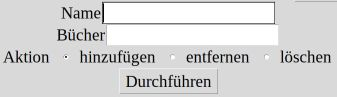
\includegraphics{images/gui2/edit_group.jpg}\caption{Die Gruppenverwaltung}\label{fig:edit_group}\end{figure}

Im Gruppenverwaltungsbereich befinden sich folgende Eingabefelder:

\begin{tabular}{|p{0.2\textwidth}|p{0.6\textwidth}|p{0.1\textwidth}|}\hline
\begin{center}Feld\end{center} & \begin{center}Bemerkung\end{center} & \begin{center}Muss angegeben werden\end{center}\\
\hline
Name & Der Name der Gruppe & Ja\\
\hline
Bücher & Die IDs der Bücher, mit denen Änderungen vorgenommen werden sollen, mit Semikolon getrennt & Nein\\
\hline
\end{tabular}

Zusätzlich befindet sich darunter ein Auswahlbereich, in dem die Art der Aktion (``hinzufügen'', ``entfernen'', ``löschen''), gewählt werden kann. Welche was bewirkt wird im Folgenden näher erläutert.

\paragraph{``hinzufügen''}
Mit dieser Aktion werden alle angegebenen Bücher der angegebenen Gruppe hinzugefügt, d.h. Gruppenaktivationen mit der angegebenen Gruppe sprechen diese Bücher ab sofort an.

\paragraph{``entfernen''}
Mit dieser Aktion werden alle angegebenen Bücher aus der angegebenen Gruppe entfernt, d.h. Gruppenaktivationen mit der angegebenen Gruppe sprechen diese Bücher ab sofort nicht mehr an.

\paragraph{``löschen''}
Mit dieser Aktion werden alle Bücher, die Teil der angegebenen Gruppe waren, aus der angegebenen Gruppe entfernt. Das ``Bücher''-Eingabefeld wird in diesem Fall ignoriert.

\hinweis{ Ich persönlich sehe wenig praktischen Nutzen für diese Aktion. Aus Symmetriegründen zur Bibliothek wird sie jedoch angeboten.}

\subsubsection{``Gruppe aktivieieren''}
\label{subsubsec:detail:edit:activate_group}
\begin{figure}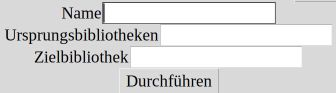
\includegraphics{images/gui2/activate_group.jpg}\caption{Die Gruppenaktivation}\label{fig:activate_group}\end{figure}

Diese Aktion besteht aus den folgenden drei Eingabefeldern:

\begin{tabular}{|p{0.15\textwidth}|p{0.45\textwidth}|p{0.1\textwidth}|p{0.2\textwidth}|}\hline
\begin{center}Feld\end{center} & \begin{center}Bemerkung\end{center} & \begin{center}Muss angegeben werden\end{center} & \begin{center}Wert, falls nicht angegeben\end{center}\\
\hline
Name & Die Namen der zu aktivierenden Gruppen, mit Semikolon getrennt & Ja &  ---\\
\hline
Ur\-sprungs\-bib\-li\-othe\-ken & Alle derzeitigen Bibliotheken, deren Bücher berücksichtigt werden sollen, mit Semikolon getrennt & Nein & alle Bibliotheken\\
\hline
Ziel\-bibliothek & Die Bibliothek, in welche die Bücher gebracht werden sollen & Nein & ``main"\\
\hline
\end{tabular}

Diese Aktion bewegt alle Bücher, die mindestens einer der angegebenen Gruppen angehören und in einer der angegebenen Ursprungsbibliotheken sind, in die Zielbibliothek.

\subsubsection{``Mitglied''}
\label{subsubsec:detail:edit:member}
\begin{figure}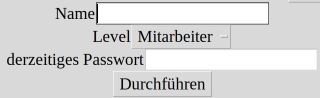
\includegraphics{images/gui2/edit_member.jpg}\caption{Die Mitgliedsverwatung}\label{fig:edit_member}\end{figure}

Diese Aktion besteht aus einem Eingabefeld für den Namen des Mitglieds und einem Auswahlmenü für das neue Level. Wird auf ``Durchführen'' geklickt, wird das Level des angegebenen Mitglieds auf das angegebene Level gesetzt. Zusätzlich muss noch das Passwort des ausführenden Mitglieds eingegeben werden. \\

\textcolor{red}{ACHTUNG: Es gibt \textbf{keinen} Schutzmechanisums, der verhindert, dass sich ein einziger Superadministrator seine Rechte nimmt.}

\hinweis{ Das Passwort eines Mitglieds kann separat unter \linkandref{subsubsec:detail:edit:change_password}{``Passwort ändern''} geändert werden.}

\subsubsection{``Passwort ändern''}
\label{subsubsec:detail:edit:change_password}
\begin{figure}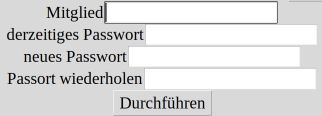
\includegraphics{images/gui2/change_password.jpg}\caption{Die Passwortänderung}\label{fig:change_password}\end{figure}

Diese Aktion besteht aus den folgenden Feldern:

\begin{tabular}{|p{0.2\textwidth}|p{0.6\textwidth}|p{0.1\textwidth}|}\hline
\begin{center}Feld\end{center} & \begin{center}Bemerkung\end{center} & \begin{center}Muss angegeben werden\end{center}\\
\hline
Name & Name des Mitglieds, dessen Password geändert werden soll & Ja\\
\hline
derzeitiges Passwort & Passwort des Mitglieds welches derzeit eingeloggt ist & Ja\\
\hline
neues Password & Neues Passwort für das angegebene Mitglied & Ja\\
\hline
Passwort wiederholen & Wiederholung des neuen Passworts & Ja\\
\hline
\end{tabular}

\hinweis{ Ein Passwort kann entweder von einem Superadministrator oder vom betroffenen Mitglied selbst geändert werden.}

\subsection{``suchen''}
\label{subsec:detail:search}
In der Suchübersicht gibt es viele Eingabefelder. Beim Suchen werden die Felder mit den Daten gefüllt, nach denen gesucht werden soll.

``Suchmodus'' kann entweder ``und'' oder ``oder'' sein. Ist er auf ``und'' gestellt, treffen alle Eingaben auf alle Ergebnisse zu; bei ``oder'' trifft auf jedes Ergebnis mindestens eine Eingabe zu.

Wird ``genaue Übereinstimmung'' gewählt, muss der tatsächliche Wert des gesuchten Objekts genau mit der Eingabe übereinstimmen, ansonsten muss die Eingabe nur im tatsächlichen Wert enthalten sein. Dies gilt nicht für Zahlen.

Bei den Bibliotheken eines Schülers und den Gruppen eines Buches kann z.Z. nur nach einem Wert gesucht werden.

% <!-- Hinweis: Die Suchfunktion wird demnauml;chst weitere Funktionalitauml;t erhalten -->
Für die Suche nach Ausleihvorgängen können Daten zum betreffenden Buch und zum betreffenden Schüler eingegeben werden.

\hinweis{ In seltenen Fällen kann es vorkommen, dass die Suchergebnisse nicht richtig angezeigt werden. In diesem Fall bitte die Taste ``q'' drücken.

Bei der Suche nach Ausleihvorgängen kann man wählen, ob das betreffende Buch bereits oder noch nicht zurückgegeben sein soll. Dabei ist die Standardauswahl (d.h. sofern nichts geändert wird) ``egal''. Mit Klick auf den Knopf kann man dann zwischen ``bereits zurück'' (gefülltes Kästchen) und ``noch nicht zurück'' (leeres Kästchen) wählen.}

\subsection{``ausleihen''}
\label{subsec:detail:borrow}
\begin{figure}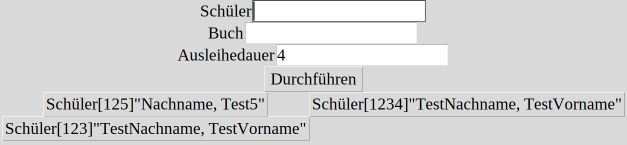
\includegraphics{images/gui2/borrow_with_people.jpg}\caption{Die Ausleihaktion. Unter den Einagbefeldern sieht man Knöpfe mit Schülern, die zuletzt ausgeliehen haben.}\label{fig:borrow_with_people}\end{figure}

Die Ausleihoberfläche besteht aus drei Eingabefeldern, die unten erläutert werden, einem mit ``Durchführen'' beschrifteten Knopf sowie ggf. weiteren Knöpfen, die mit Kurzdarstellungen einiger Schüler beschriftet sind.
Wird einer dieser Knöpfe gedrückt, wird das angegebene Buch an den auf dem Knopf stehenden Schüler ausgeliehen. Der Wert im Schüler-Eingabefeld wird dann automatisch gefüllt.

Die Eingabefelder:

\begin{tabular}{|p{0.15\textwidth}|p{0.35\textwidth}|p{0.4\textwidth}|}\hline
\begin{center}Feld\end{center} & \begin{center}Bemerkung\end{center} & \begin{center}Muss angegeben werden\end{center}\\
\hline
Schüler & Die Schülerausweisnummer des Schülers, an den das Buch ausgeliehen werden soll & Ja, außer es wird ein Knopf mit Schüler gedrückt\\
\hline
Buch & Die ID des auszuleihenden Buches & Ja\\
\hline
Zeitraum & Wie viele Wochen das Buch ausgeliehen werden soll & Ja\\
\hline
\end{tabular}

\subsection{``zurückgeben''}
\label{subsec:detail:restitute}
\begin{figure}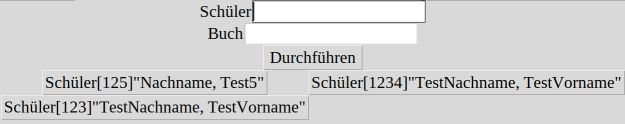
\includegraphics{images/gui2/restitute_with_people.jpg}\caption{Die Rückgabeaktion. Unter den Einagbefeldern sieht man Knöpfe mit Schülern, die zuletzt ausgeliehen haben.}\label{fig:restitute_with_people}\end{figure}


Die Rückgabeoberfläche besteht aus einem Eingabefeld für die Schülerausweisnummer des zurückgebenden Schülers und ein Eingabefeld für die ID des zurückgegebenen Buches. Darunter befindet sich ein mit ``Durchführen'' beschrifteter Knopf sowie ggf. weitere, mit Kurzdarstellungen von Schülern beschriftete, Knöpfe.

Wird der ``Durchführen''-Knopf gedrückt, müssen beide Eingabefelder gefüllt sein; das angegebene Buch wird als zurückgegeben vermerkt.

Wird einer der anderen Knöpfe gedrückt, wird das angegebene Buch als zurückgegeben vermerkt, wobei als ausleihender Schüler der auf dem Knopf beschriebene genommen wird.

\hinweis{Die Schülerausweisnummer wird abgefragt, um Probleme durch Vertippen bei Eingabe der Buch-ID zu verhindern. 
Bei Unstimmigkeitenwird eine Fehlermeldung angezeigt.
Sollte nicht bekannt sein, wer ein Buch ausgeliehen hat, kann dies durch die\linkandref{subsubsec:detail:view:book}{ ``betrachten'' $\rightarrow$ ``Buch''-Aktion} eingesehen werden.
Alternativ ist es in der Textoberfläche möglich, eine Rückgabe durchzuführen, ohne dass eine Schülerausweis-Nr. benötigt wird.}

\end{document}